% Color of bar plot depending on the bar height (pgfplot)
% https://tex.stackexchange.com/questions/132081/color-of-bar-plot-depending-on-the-bar-height-pgfplot?noredirect=1&lq=1
\documentclass{standalone}
\usepackage{pgfplots,pgfplotstable}

\begin{document}
	
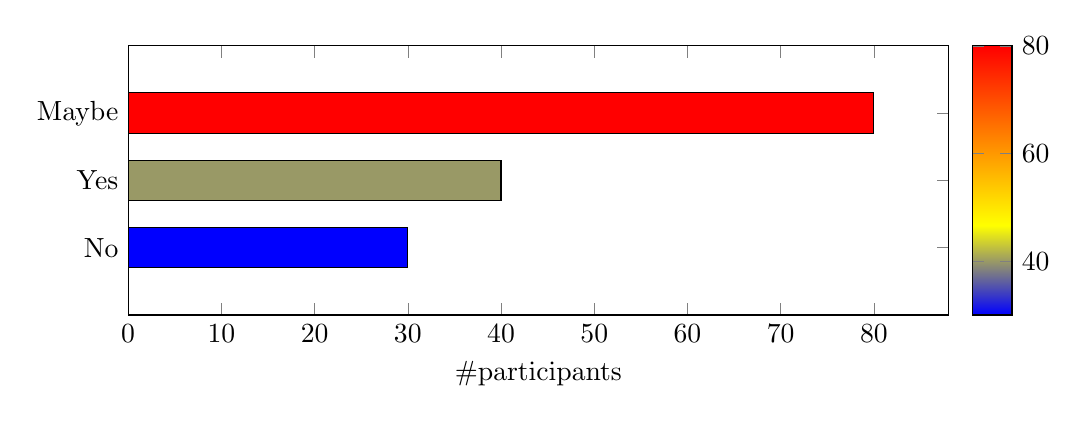
\begin{tikzpicture}
  \begin{axis}[
      colorbar,
    point meta min=30, point meta max=80,
    only marks,
    scatter,
    scatter src=x,
    clip mode=individual,
    scatter/@pre marker code/.append code={
            \pgfkeys{/pgf/fpu=true,/pgf/fpu/output format=fixed}
            \pgfmathsetmacro\negheight{-\pgfplotspointmeta}         
            \fill [draw=black] (axis direction cs:0,0.3) rectangle (axis direction cs:\negheight,-0.3);
            \pgfplotsset{mark=none}
        },
    xmin=0,
    width=12cm, height=5cm, enlarge y limits=0.5,
    xlabel={\#participants},
    ytick=data,
    yticklabels={No, Yes, Maybe}
    ]
    \addplot table [y expr=\coordindex] {
    Participants Answer
    30 no
    40 yes
    80 maybe
    };
  \end{axis}
\end{tikzpicture}
\end{document}
